\documentclass{beamer}
\usetheme{Madrid}
\usepackage{amsmath,amssymb}
\usepackage{array}
\usepackage{longtable}

\title{Problem 9.4.7}
\author{AI25BTECH11035- SUJAL RAJANI}
\date{\today}

\begin{document}

\begin{frame}
  \titlepage
\end{frame}

% Question Slide
\begin{frame}{Question}
  \textbf{Question:} Find the roots of the following quadratic equation graphically:
  \[
    16x^2 - 8x + 1 = 0
  \]
\end{frame}

% Solution: Standard Form
\begin{frame}{Solution}
First, the equation is already in standard quadratic form:
\[
  16x^2 - 8x + 1 = 0
\]

\textbf{Input Variables:}

The given quadratic can be written in the conic form:
\[
  \vec{x}^T\vec{V}\vec{x} + 2\vec{u}^T\vec{x} + f = 0
\]
where
\[
  \vec{V} = \begin{pmatrix} 16 & 0 \\ 0 & 0 \end{pmatrix}, \quad
  \vec{u} = \begin{pmatrix} -4 \\ 0 \end{pmatrix}, \quad
  f = 1
\]
\end{frame}

% Solution: Line Representation
\begin{frame}{Solution}
Since the roots correspond to intersections with the x-axis, we represent the line:
\[
  L : \vec{x} = \vec{h} + \kappa\vec{m}
\]
with
\[
  \vec{h} = \begin{pmatrix} 0 \\ 0 \end{pmatrix}, \quad
  \vec{m} = \begin{pmatrix} 1 \\ 0 \end{pmatrix}
\]
\end{frame}

% Table of Input Parameters
\begin{frame}{Input Parameters}
\begin{table}[h]
\centering
\begin{tabular}{|c|c|}
\hline
\textbf{Symbol} & \textbf{Value} \\
\hline
$\vec{V}$ & $\begin{pmatrix} 16 & 0 \\ 0 & 0 \end{pmatrix}$ \\
\hline
$\vec{u}$ & $\begin{pmatrix} -4 \\ 0 \end{pmatrix}$ \\
\hline
$f$ & $1$ \\
\hline
$\vec{h}$ & $\begin{pmatrix} 0 \\ 0 \end{pmatrix}$ \\
\hline
$\vec{m}$ & $\begin{pmatrix} 1 \\ 0 \end{pmatrix}$ \\
\hline
\end{tabular}
\caption{Input Parameters}
\end{table}
\end{frame}

% Intersection with Conic
\begin{frame}{Solution}
The points of intersection of a line with a conic are:
\[
  \kappa = \frac{1}{\vec{m}^T\vec{V}\vec{m}}
  \left[
    -\vec{m}^T(\vec{V}\vec{h}+\vec{u}) \pm 
    \sqrt{
      \left[\vec{m}^T(\vec{V}\vec{h}+\vec{u})\right]^2
      - g(\vec{h})\vec{m}^T\vec{V}\vec{m}
    }
  \right]
\]
where
\[
  g(\vec{h}) = \vec{h}^T\vec{V}\vec{h} + 2\vec{u}^T\vec{h} + f
\]
\end{frame}

% Step-by-step Calculation
\begin{frame}{Step-by-Step Evaluation}
\textbf{Step 1:} Compute $\vec{m}^T\vec{V}\vec{m}$
\[
  \vec{m}^T\vec{V}\vec{m} = 16
\]
\textbf{Step 2:} Compute $\vec{V}\vec{h} + \vec{u}$
\[
  \vec{V}\vec{h} + \vec{u} = \begin{pmatrix} -4 \\ 0 \end{pmatrix}
\]
\textbf{Step 3:} Compute $\vec{m}^T(\vec{V}\vec{h}+\vec{u})$
\[
  \vec{m}^T(\vec{V}\vec{h}+\vec{u}) = -4
\]
\textbf{Step 4:} Compute $g(\vec{h})$
\[
  g(\vec{h}) = 1
\]
\end{frame}

% Substitute and Final Root
\begin{frame}{Final Roots}
\textbf{Step 5:} Substitute into $\kappa$:
\[
  \kappa = \frac{4 \pm \sqrt{16-16}}{16} = \frac{4}{16} = 0.25
\]
\textbf{Step 6:} Intersection point:
\[
  x = h + \kappa m = (0,0) + (0.25)(1,0) = (0.25, 0)
\]
Thus, the quadratic $16x^2 - 8x + 1 = 0$ intersects the x-axis at
\[
  \boxed{x = 0.25}
\]
\end{frame}
      \begin{frame}[fragile]
    \begin{figure}[H]
    \centering
    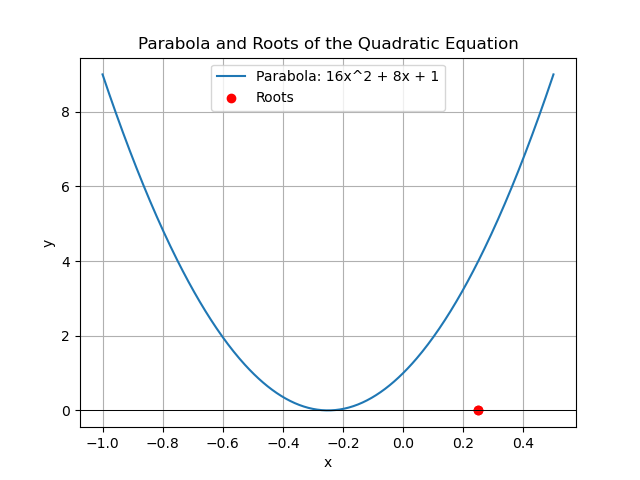
\includegraphics[width = 0.6\columnwidth]{../figs/img.png}
    \caption*{}
    \label{figs}
\end{figure}
\end{frame}

\end{document}
